% ju 13-Aug-22
\documentclass[a4paper,12pt,fleqn,parskip=half]{scrartcl}
\usepackage[ngerman]{babel}
\usepackage[utf8]{inputenc}
\usepackage[T1]{fontenc}

% Schrift
%\usepackage{lmodern}
\usepackage[osf,sc]{mathpazo} 
\usepackage[scale=.9,semibold]{sourcecodepro}   
\usepackage[osf]{sourcesanspro}  

\usepackage[headsepline]{scrlayer-scrpage}
\pagestyle{scrheadings}
\clearpairofpagestyles

\usepackage[table,dvipsnames,usenames]{xcolor}
\usepackage{textcase}
\usepackage{nameref}
\usepackage{hyperref}
\usepackage{tabularx}
\usepackage{multirow}
\usepackage{multicol}
\usepackage{caption, booktabs}
\usepackage{graphicx} 
\usepackage{scrhack}    
\usepackage{url}%% Links
\usepackage[inline]{enumitem}
\usepackage{pifont}
\usepackage{eurosym}% \euro 20,-
\usepackage{amsmath}
\usepackage{amsfonts}
\usepackage{amssymb}
\usepackage{array}            % Extending the array and tabular environments
\usepackage{chngcntr}         % Change the resetting of counters
\usepackage[version=4]{mhchem}
\usepackage{stmaryrd}
\usepackage{siunitx}
\usepackage{float}
\usepackage{csquotes}
\usepackage{subcaption}
\usepackage{mathtools}
\usepackage{icomma}%Dezimaltrennzeichen
\usepackage{multimedia}%Video: \movie[externalviewer]{(video.mov)}{video.mov}
\usepackage{epstopdf}
\usepackage{footnote}
\usepackage{qrcode}% Anwendung: \qrcode[hyperlink,level=Q,version=2,height=1cm]{\website}
\usepackage{underscore}% Unterstrich ____

% PDF Dokumente einbinden
\usepackage{pdfpages}% \includepdf[pages=-]{Tabellen/Excel.pdf}
\RequirePackage{lastpage}  % Pagecounter

\addto\captionsngerman{%
\renewcommand{\figurename}{Abb.}
\renewcommand{\tablename}{Tab.}
}

% listings
\usepackage{listings}
\lstset{basicstyle=\linespread{1}\ttfamily\small,floatplacement=!htb,captionpos=t,abovecaptionskip=.5\baselineskip,belowcaptionskip=.5\baselineskip,upquote=true,showstringspaces=false,inputencoding=utf8,tabsize=4,
    	keywordstyle=\bfseries ,
	commentstyle=\color{rot5},
	stringstyle=\color{orange},
	breaklines=true,
  	postbreak=\mbox{\textcolor{black}{$\hookrightarrow$}\space},
	breakatwhitespace=false
}
\lstset{literate={á}{{\'a}}1 {é}{{\'e}}1 {í}{{\'i}}1 {ó}{{\'o}}1 {ú}{{\'u}}1 {Á}{{\'A}}1 {É}{{\'E}}1 {Í}{{\'I}}1 {Ó}{{\'O}}1 {Ú}{{\'U}}1 {à}{{\`a}}1 {è}{{\`e}}1 {ì}{{\`i}}1 {ò}{{\`o}}1 {ù}{{\`u}}1 {À}{{\`A}}1 {È}{{\'E}}1 {Ì}{{\`I}}1 {Ò}{{\`O}}1 {Ù}{{\`U}}1 {ä}{{\"a}}1 {ë}{{\"e}}1 {ï}{{\"i}}1 {ö}{{\"o}}1 {ü}{{\"u}}1 {Ä}{{\"A}}1 {Ë}{{\"E}}1 {Ï}{{\"I}}1 {Ö}{{\"O}}1 {Ü}{{\"U}}1 {â}{{\^a}}1 {ê}{{\^e}}1 {î}{{\^i}}1 {ô}{{\^o}}1 {û}{{\^u}}1 {Â}{{\^A}}1 {Ê}{{\^E}}1 {Î}{{\^I}}1 {Ô}{{\^O}}1 {Û}{{\^U}}1 {œ}{{\oe}}1 {Œ}{{\OE}}1 {æ}{{\ae}}1 {Æ}{{\AE}}1 {ß}{{\ss}}1 {ű}{{\H{u}}}1 {Ű}{{\H{U}}}1 {ő}{{\H{o}}}1 {Ő}{{\H{O}}}1 {ç}{{\c c}}1 {Ç}{{\c C}}1 {ø}{{\o}}1 {å}{{\r a}}1 {Å}{{\r A}}1 {€}{{\EUR}}1 {£}{{\pounds}}1 {~}{{\textasciitilde}}1 {-}{{-}}1 }

% bibliography
\usepackage[
    bibencoding=utf8,
    backend=biber,% bibtex, biber
    backref=false,backrefstyle=three+,url=true,urldate=comp,abbreviate=false,maxnames=20
]{biblatex} %Paket laden
\DeclareBibliographyCategory{cited}
\let\defaultcite\cite\renewcommand*\cite[2][]{\addtocategory{cited}{#2}\defaultcite[#1]{#2}}
\let\defaulttextcite\textcite\renewcommand*\textcite[2][]{\addtocategory{cited}{#2}\defaulttextcite[#1]{#2}}
\setcounter{biburllcpenalty}{7000}
\setcounter{biburlucpenalty}{8000}
\AfterPackage{biblatex}{
	\PreventPackageFromLoading[\errmessage{Sie haben versucht, das Cite-Paket zu laden, das nicht mit biblatex kompatibel ist.}]{cite}
}

\hypersetup{%
	%pdftitle={\titel},
	%pdfsubject={Latex},
	%pdfauthor={\autor},
	%pdfcreator={\autor}, 
	bookmarksnumbered=true,
	breaklinks=true,
	%colorlinks=true,	   
	linkcolor=rot5,		
	filecolor=blau5,		
	urlcolor=blau5,			
	citecolor=ForestGreen
}

\linespread{1.1}
\setlist{itemsep=0pt}
\widowpenalty10000
\clubpenalty10000
\tolerance1000   

\usepackage[left=2cm,right=2cm,top=1cm,bottom=1cm,includeheadfoot]{geometry}
%\usepackage[left=4cm,right=2cm,top=1cm, bottom=1cm,includeheadfoot]{geometry}
%\usepackage[left=6cm,right=1cm,top=1cm, bottom=1cm,includeheadfoot]{geometry}
%\usepackage[landscape=true,left=2cm,right=2cm,top=1cm,bottom=1cm,includeheadfoot]{geometry}%quer

% eigene Farbe definieren
% Adobe Prozessfarben: CMYK: 100,50,0,35 -> 1,0.5,0,0.35
\definecolor{orange}{cmyk}{0,0.55,0.61,0}   % 0,55,61,0
\definecolor{blau5}{cmyk}{1,0.77,0.1,0.01}  % 100,77,10,
\definecolor{rot5}{cmyk}{0.22,1,1,0.19}     % 22,100,100,19
\definecolor{grau2}{cmyk}{0,0,0,0.1}        % 0,0,0,40
\definecolor{blau}{cmyk}{0.93,0.66,0,0.21}% 

% Literatur
\bibliography{content/literatur}
\bibliography{content/literatur-kfz}
\bibliography{content/literatur-sport}

%%%%%%%%%%%%%%%%%%%%%%%%%%%%%%%%%%%%%%%%%%%%%%%%%%%%%%%
\newcommand{\name}{Jan Unger}
\newcommand{\thema}{06-Klimaanlage}
\newcommand{\quelle}{\name}
\newcommand{\website}{https://bw-ju.de/}
\newcommand{\github}{https://github.com/ju1-eu}
%%%%%%%%%%%%%%%%%%%%%%%%%%%%%%%%%%%%%%%%%%%%%%%%%%%%%%%

\ihead{\textbf{Quelle:} \quelle}%{Kopfzeile innen}
\ohead{\textbf{Datum:} \today}  %{Kopfzeile außen}
\ifoot{\textbf{Thema:} \thema}  %{Fußzeile  innen}
\ofoot{Seite {\thepage} von {\pageref{LastPage}}}%{Fußzeile  außen}

\title{\thema}
\author{\name}
\date{\today}

\begin{document}
	%%%%%%%%%%%%%%%%%%%%%%%%%%%%%%%%%%%%%%%%%%%%%%%%%%%%%%%%%%%%%%%%%%
	\begin{abstract}
		\center
		\textbf{\Large \thema}%14pt
		
		\vspace{1.5em}
		%\datum	
		%\qrcode[hyperlink,level=Q,version=2,height=1cm]{\website}
		\qrcode[hyperlink,level=Q,version=2,height=1cm]{\github}
		
		\vspace{1.5em} 
		\raggedright
		\textbf{\large Keywords}
		% Checkliste
		\begin{itemize}[label=\checkmark]
			\item Begriff
		\end{itemize}
	\end{abstract}
    %%%%%%%%%%%%%%%%%%%%%%%%%%%%%%%%%%%%%%%%%%%%%%%%%%%%%%%%%%%%%%%%%%

	% anpassen
	%\input{content/tex/neu}
	%ju 26-Dez-22 06-Klimaanlage.tex
\section{Aktive und Passive
Sicherheit}\label{aktive-und-passive-sicherheit}

\textbf{Aktive Sicherheit} Maßnahmen zur Vermeidung von Unfällen

\begin{itemize}
\item
  \emph{Beispiele:} ABS, ESP, Klima, Scheibenwischer, ACC (adaptive
  Geschwindigkeitsregelung)
\end{itemize}

\emph{Klima}: die Raumtemperatur wird runtergekühlt, Aufmerksamkeit
steigt und der Pollenfilter bewirkt eine geringere Allergie last für
Allergiker.

\textbf{Passive Sicherheit} Maßnahmen zur Minderung von Unfallfolgen

\begin{itemize}
\item
  \emph{Beispiele:} Airbag (Fahrer-, Beifahrer-, Kopf- und
  Seitenairbags), Gurtstraffer, Batterietrennschalter (Kurzschluss,
  Brandgefahr), Motorhaubenaufsteller
\end{itemize}

\textbf{Airbag löst nach} ca. $15 - 50~ms$ aus (Zündung --
Entfaltung), Crashsensoren: max. $30^\circ$ Aufprallwinkel zur
Längsachse

\textbf{Gurtstraffer zieht Gurt nach} ca. $20 - 25~ms$ bis zu
$15~cm$ ein.

\newpage

\section{Aufbau und Funktionsweise einer
Klimaanlage}\label{aufbau-und-funktionsweise-einer-klimaanlage}

\textbf{Luftgütesensor:} misst Schadstoffe in der Außenluft (Frischluft
vs.~Innenraumluft)

\textbf{Wärme} vs.~\textbf{geringe, hohe Wärme, Wärmeentzug} (Kälte gibt
es in der Physik nicht)

\textbf{Enthalpie} Element, das eine bestimmte Wärmeenergie hat

\subsection{Komponenten}\label{komponenten}

\begin{enumerate}
\item
  \textbf{Magnetkupplung} Verbindung zwischen Riemenscheibe und
  Antriebswelle

  \begin{itemize}
  \item
    Spaltmaß: $0,4 - 0,6~mm$
  \end{itemize}
\item
  \textbf{Kompressor} Kältemittel verdichten

  \begin{itemize}
  \item
    Taumelscheibenverdichter (Förderleistung variieren)
  \item
    Flügelzellenverdichter
  \item
    Spiralverdichter (Hybrid- und Elektrofahrzeuge)
  \item
    Kompressor mit variablem Hub und externer Regelung (PWM-Signal)
  \end{itemize}
\item
  \textbf{Trockner} flüssiges Kältemittel wird entfeuchtet und
  gefiltert, beruhigen, Sammler
\item
  \textbf{Expansionsventil} regelt Kältemittelzufluss zum Verdampfer, um
  zu verhindern, dass der Kompressor flüssiges Kältemittel ansaugt
  (Flüssigkeitsschlag)
\item
  \textbf{Druckschalter und Überdruckventil} Schutz der Klimaanlage

  \begin{itemize}
  \item
    Kühlerlüfter / Kondensatorgebläse

    \begin{itemize}
    \item
      EIN: $\sim 16~\text{bar}$, AUS: $\sim 10~\text{bar}$
    \end{itemize}
  \item
    Magnetkupplung

    \begin{itemize}
    \item
      Druckschalter: Druck zu niedrig $\sim 2~\text{bar}$, Druck zu
      hoch $\sim 28~\text{bar}$
    \end{itemize}
  \item
    Verdampfersonde / Vereisungssensor

    \begin{itemize}
    \item
      Vereisungsschutz EIN $> +4^\circ \text{C}$, AUS
      $< 0^\circ \text{C}$
    \end{itemize}
  \end{itemize}
\end{enumerate}

\subsection{Funktion des
Kältemittels}\label{funktion-des-kaeltemittels}

Kältemittel nimmt Energie auf und gib sie wieder ab bei Änderung seines
Aggregatzustandes.

Bei geringem Druck und niedriger Temperatur verdampft Kältemittel. Der
Siedepunkt kann durch Druckänderung verschoben werden. Erhöht man den
Druck, dann steigt die Verdampfungstemperatur.

Beispiel: R134a

\begin{itemize}
\item
  Atmosphärische Druck: ca. $1~\text{bar} \to$ Siedepunkt: ca.
  $-26^\circ \text{C}$
\item
  Überdruck: ca. $15~\text{bar} \to$ Siedepunkt: ca.
  $55^\circ \text{C}$
\end{itemize}

\textbf{Verdampfer} verdampfen, Energie aufnehmen (\emph{Wärme\_zu}) aus
der Umgebung wird Wärme entzogen. Notwendig, wenn man eine Flüssigkeit
verdampfen möchte. (flüssig $\to$ gasförmig)

vs.

\textbf{Kondensator} kondensieren, Energie abgeben (\emph{Wärme\_ab}) an
die Umgebung (gasförmig $\to$ flüssig)

\textbf{Wärmepumpe} Heizen (PTC) und Kühlen

\newpage

\subsection{Erkläre den
Kältemittelkreislauf}\label{erklaere-den-kaeltemittelkreislauf}

\begin{figure}[!ht]% hier: !ht
\centering
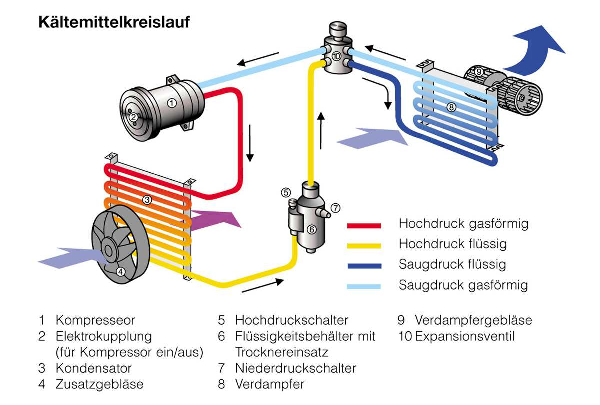
\includegraphics[width=0.7\textwidth]{images/Klima/Klimakreislauf-1.pdf}
\caption{Klimakreislauf}
%\label{fig:}%% anpassen
\end{figure}

\begin{enumerate}
\item
  \textbf{Kompressor} (Gasverdichter, gasförmig, Verdichten, Druck
  steigt) saugt das abgekühlte gasförmige Kältemittel an und verdichtet
  es. Druck und Temperatur steigt (Druckanstieg). Das Kältemittel
  erwärmt sich, wird aber nicht komplett flüssig. Deshalb schieben wir
  es durch den Kondensator.
\item
  \textbf{Kondensator} (Verflüssiger, Kondensieren) hier wird das
  Kältemittel von der Umgebungsluft durchströmt und abgekühlt.
  Aggregatzustand wechsel von gasförmig $\to$ flüssig (Druck ist
  konstant). Kältemittel wird flüssig, wenn es den Kondensator verlässt.
\item
  \textbf{Expansionsventil} (Dosiereinheit, Druckminderer, Drossel,
  Expandieren, flüssig) Kältemittel expandiert durch die Drossel (Druck
  abfall) und lässt bedarfsgerecht eine bestimmte definierte Menge
  Kältemittel durch Strömen.
\item
  \textbf{Verdampfer} (Verdampfen) dadurch wird ein Aggregatzustand
  wechsel von flüssig $\to$ gasförmig (Druck ist konstant)
  gewährleistet. Die durch den Verdampfer strömende Umgebungsluft
  runterkühlen und in den Innenraum einströmen lassen. Dabei entzieht
  das Kältemittel der Umgebungsluft Wärme und kühlt sie ab.
\end{enumerate}

\newpage

\subsection{Kunde bemängelt, Klimaanlage kühlt nicht
richtig}\label{kunde-bemaengelt-klimaanlage-kuehlt-nicht-richtig}

\textbf{Es wurde beispielsweise nur 100 g Kältemittel abgesaugt. Kann
die Klimaanlage wieder befüllt werden?}

Nicht befüllen $\to$ wir machen uns strafbar.

Kältemittel absaugen und mit Stickstoff auf Undichtigkeit prüfen.

\textbf{Verlust an Kältemittel}
$[\%] \, \boxed{= \frac{\text{abgesaugte Menge}}{\text{Füllmenge}} \cdot 100} \quad \text{Beispiel: } \frac{180~g}{640~g} \cdot 100 = 28~\%$

Jährlich ca. $10~\%$ Verlust normal.

\subsection{Was ist der Unterschied zwischen intern und extern geregelte
Klimakompressoren?}\label{was-ist-der-unterschied-zwischen-intern-und-extern-geregelte-klimakompressoren}

\textbf{Intern}, die Stellung der Taumelscheibe und damit die
Fördermenge wird durch ein Regelventil bestimmt. Kann bei Bedarf über
eine Magnetkupplung entkoppelt und damit komplett ausgeschaltet werden.

\emph{Nachteil:} >>kaputt stehen<< eine Klimaanlage nimmt Schaden, wenn
sie nicht regelmäßig eingeschaltet wird (Dichtungen, Schmierung)

\textbf{Extern} keine Magnetkupplung, mit Überlastschutz, Anlage läuft
immer, aber Fördermenge wird runtergeregelt auf ca. $2~\%$

\emph{Nachteil:} Reibung

\subsection{Kältemittel R744 - Problem bei hohen
Außentemperaturen}\label{kaeltemittel-r744-problem-bei-hohen-aussentemperaturen}

Klima funktioniert schlecht bei zu hohen Außentemperaturen
$> 35^\circ\text{C}$. Kältemittel wird nicht genug runtergekühlt.

\subsection{Warum sollte man eine Klimaanlage spülen und welche
Möglichkeiten gibt
es?}\label{warum-sollte-man-eine-klimaanlage-spuelen-und-welche-moeglichkeiten-gibt-es}

Bei Verunreinigungen, Beispiel Kompressor schaden.

\begin{itemize}
\item
  Sieb Einsätze
\item
  Formiergas, Stickstoff, mit Kältemittel (Quelle: Andreas Lamm)
\end{itemize}

\textbf{Offene Anlage} Trockner erneuern oder Anlage verschließen.

\subsection{Desinfizieren einer
Klimaanlage}\label{desinfizieren-einer-klimaanlage}

\begin{itemize}
\item
  Ozongeräte (24h)
\item
  Spray (geringe Wirkung)
\end{itemize}

\subsection{Warum läuft aus der Klimaanlage Wasser bei heißem
Wetter?}\label{warum-laeuft-aus-der-klimaanlage-wasser-bei-heissem-wetter}

\begin{itemize}
\item
  \textbf{Sommer} schwüles Wetter hat eine hohe Luftfeuchtigkeit
\item
  \textbf{Winter} kalte Luft hat eine geringe Luftfeuchtigkeit
\end{itemize}

\subsection{Welche Kältemittelöle gibt es und wo ist der
Unterschied?}\label{welche-kaeltemitteloele-gibt-es-und-wo-ist-der-unterschied}

Herstellerangaben befolgen - Typenschild auf dem Klimakompressor

\begin{itemize}
\item
  \textbf{PAG-Öle} hygroskopisch
\item
  \textbf{POE-Öle} Polyester-Öl, elektrisch isolierendes
  Klimakompressoröl
\end{itemize}

\newpage

\section{Klimaservice}\label{klimaservice}

\textbf{Ruhedruck} (Motor aus)

\begin{itemize}
\item
  Kältemitteldruck abhängig von Umgebungstemperatur (Vgl. Dampftafel /
  Richtwerte \textcite{schmidt:2015:klima} S. 120)
\end{itemize}

\textbf{Betriebsdruck} (Motor an im LL, Klima ON, max. Gebläse, keine
Umluft, Heizung OFF, Temp. LOW, $5 - 10~\text{Min.}$ laufen lassen)

\begin{itemize}
\item
  \textbf{Sollwerte} Quelle: Andreas Lamm \footnote{\url{https://klimacheck.com/}}
\item
  ND $1 - 3~\text{bar}$
\item
  HD $7 - 20~\text{bar}$
\item
  Kühlung

  \begin{itemize}
  \item
    Außentemperatur $20^\circ \text{C} \to 2 - 8^\circ \text{C}$
    \textbf{Ausströmtemperatur}
  \item
    Außentemperatur $30^\circ \text{C} \to \, <15^\circ \text{C}$
    Ausströmtemperatur
  \end{itemize}
\end{itemize}

\subsection{Klimadiagnose}\label{klimadiagnose}

\begin{enumerate}
\item
  Betriebsdruck (Vgl. Sollwerte)

  \begin{itemize}
  \item
    \textbf{Läuft Kondensatorlüfter?}

    \begin{itemize}
    \item
      Wenn Defroster EIN, dann muss Lüfter laufen!
    \end{itemize}
  \end{itemize}
\item
  Ausströmtemperatur (Vgl. Sollwerte)
\item
  Zustand Kältemittel (Schauglas)
\end{enumerate}

\emph{Vgl. Diagnosetabelle}

\begin{table}[!ht]% hier: !ht 
\centering 
	\caption{}% \label{tab:}%% anpassen 
\begin{tabular}{@{}lll@{}}
\hline
\textbf{Hochdruck} & \textbf{Niederdruck} & \textbf{Ursache} \\
\hline
normal, zu hoch & zu niedrig & Expansionsventil, Filter, Kondensator \\
normal, zu niedrig & zu hoch & zu viel Kältemittel, Kompressor \\
normal, zu niedrig & zu niedrig & zu wenig Kältemittel,
Magnetkupplung \\
zu niedrig & zu hoch & zu viel Kältemittel, Kondensator,
Kondensatorlüfter \\
\hline
\end{tabular} 
\end{table}

Anhand der Leitungstemperaturen auf mögliche Defekte im
Kältemittelkreislauf schließen (\textcite{schmidt:2015:klima} S. 115).

Übersicht über fehlerhafte Füllmengen und Komponenten, die sich an den
Druckmanometern widerspiegeln können (\textcite{schmidt:2015:klima} S. 116
-- 117).

\subsection{Magnetkupplung und Kondensatorlüfter
prüfen}\label{magnetkupplung-und-kondensatorluefter-pruefen}

\textbf{Magnetkupplung am Kompressor prüfen}

\begin{enumerate}
\item
  Spannungsversorgung prüfen (Verkabelung, Sicherung, Relais)

  \begin{enumerate}
  \def\labelenumii{\arabic{enumii}.}
  \item
    Magnetkupplung (Spannung am Verbraucher) Soll: $12~V$
  \item
    Masseanschluss (gegen Masse) Soll: $0~V$
  \item
    Relais (gegen Masse) Soll: $12~V$
  \item
    Druckschalter (gegen Masse) Soll: $12~V$
  \end{enumerate}
\item
  Temperatur- und Druckschalter, Steuergerät, Luftspalt
\end{enumerate}

\textbf{Kondensatorlüfter prüfen}

\begin{itemize}
\item
  Sicherung, Relais, Verkabelung, Motor, schwergängig
\end{itemize}

\subsection{Klima-Service-Gerät}\label{klima-service-geraet}

\begin{itemize}
\item
  Vakuumzeit
  $\boxed{60~Min/kg \cdot \text{Kältemittelmenge [kg]}} \quad (1~h~\hat =~ 1~kg)$
\item
  Füllung
\item
  Kompressor-Öl
\end{itemize}

Phasen

\begin{enumerate}
\item
  \textbf{Absaugen} (von Kältemittel und Kompressoröl)
\item
  \textbf{Evakuieren} (Vakuum, Wasser entfernen, Dichtigkeit prüfen)
\item
  \textbf{Aufbereiten} (Kältemittel von Wasser und Öl trennen und
  wiegen)
\item
  \textbf{Auffüllen} (von Kältemittel und Kompressoröl)
\end{enumerate}


	%%%%%%%%%%%%%%%%%%%%%%%%%%%%%%%%%%%%%%%%%%%%%%%%%%%%%%%%%%%%%%%%%%
    % Bibliographie
    \printbibliography[category=cited]
\end{document}
